\begin{figure}[tbp]
\centering
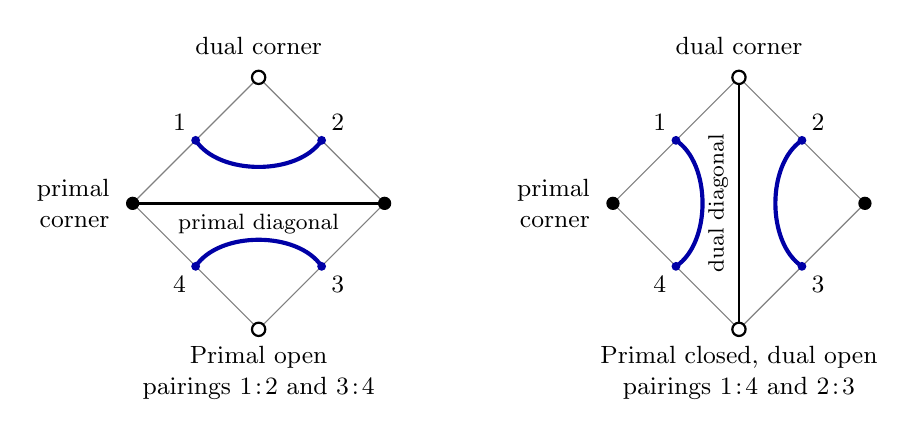
\begin{tikzpicture}[x=1cm,y=1cm,font=\small,line cap=round,line join=round]
  \foreach \shift in {0,6.1} {
    \begin{scope}[xshift=\shift cm]
      \draw[gray] (-1.6,0) -- (0,1.6) -- (1.6,0) -- (0,-1.6) -- cycle;
      \node[above] at (0,1.77) {dual corner};
      \node[left,align=right] at (-1.77,0) {primal\\corner};
      \node[above left] at (-.8,.8) {$1$};
      \node[above right] at (.8,.8) {$2$};
      \node[below right] at (.8,-.8) {$3$};
      \node[below left] at (-.8,-.8) {$4$};
    \end{scope}
  }
  \draw[line width=1pt] (-1.6,0) -- (1.6,0);
  \node[below,font=\footnotesize] at (0,-.015) {primal diagonal};
  \draw[blue!65!black,line width=1.5pt]
    (-.8,.8) .. controls (-.5,.35) and (.5,.35) .. (.8,.8);
  \draw[blue!65!black,line width=1.5pt]
    (-.8,-.8) .. controls (-.5,-.35) and (.5,-.35) .. (.8,-.8);
  \begin{scope}[xshift=6.1cm]
    \draw[line width=1pt] (0,-1.6) -- (0,1.6);
    \node[rotate=90,above,font=\footnotesize] at (-.015,0) {dual diagonal};
    \draw[blue!65!black,line width=1.5pt]
      (-.8,.8) .. controls (-.35,.5) and (-.35,-.5) .. (-.8,-.8);
    \draw[blue!65!black,line width=1.5pt]
      (.8,.8) .. controls (.35,.5) and (.35,-.5) .. (.8,-.8);
  \end{scope}
  \foreach \shift in {0,6.1} {
    \begin{scope}[xshift=\shift cm]
      \fill (-1.6,0) circle (2.4pt);
      \fill (1.6,0) circle (2.4pt);
      \draw[fill=white,line width=.8pt] (0,1.6) circle (2.4pt);
      \draw[fill=white,line width=.8pt] (0,-1.6) circle (2.4pt);
      \foreach \x/\y in {-.8/.8,.8/.8,.8/-.8,-.8/-.8}
        \fill[blue!65!black] (\x,\y) circle (1.6pt);
    \end{scope}
  }
  \node[align=center] at (0,-2.15)
    {Primal open\\pairings $1\!:\!2$ and $3\!:\!4$};
  \node[align=center] at (6.1,-2.15)
    {Primal closed, dual open\\pairings $1\!:\!4$ and $2\!:\!3$};
\end{tikzpicture}
\caption{The two local switch states, with ports numbered clockwise. Black dots are primal corners and white dots are dual corners. The black diagonal is the open physical bond; the complementary diagonal is omitted. Blue curves are medial strands: an open primal bond pairs ports around the dual corners, while an open dual bond pairs ports around the primal corners. The switch drawing records the same FK edge state and introduces no additional randomness.}
\label{fig:local-switch}
\end{figure}
